
%%%%%%%%%%%%%%%%%%%%%%%%%%%%%%%%%%%%%%%%%%%%%%%%%%%%%%%%%%%%%%%%%%%%%%%%%%%%%%%%
%% CAPITULO
%%%%%%%%%%%%%%%%%%%%%%%%%%%%%%%%%%%%%%%%%%%%%%%%%%%%%%%%%%%%%%%%%%%%%%%%%%%%%%%%
\chapterimage{chapter_head_2.pdf} % Chapter heading image

\chapter{Historia do samba de gafieira  (dança)}
\label{cap:sambagafieira}
\index{Dança!Samba de gafieira}


\section{Lundum (a dança do lundu)} 
\label{sec:lundu}
\index{Dança!Lundu}
O lundum é o estilo de dança que lhe corresponde ao gênero musical lundu \cite[pp. 18]{perna2002samba}.
Esta é uma dança, brasileira, de roda e umbigada; e teve sua origem no batuque dos bantos africanos,
e provavelmente foi trazida de Angola pelos escravos na segunda metade do século XVIII 
\cite[pp. 48]{tinhorao1986pequena} \cite[pp. 188]{dourado2004dicionario},
sendo que as primeiras referencias conhecidas se remontam a 1780 
descrevendo a dança como indecente e licenciosa \cite[pp. 51]{tinhorao1986pequena} \cite[pp. 19]{perna2002samba}.
Posteriormente foi introduzida aos salões das cortes do Brasil e Portugal, 
dançado elegantemente nas cortes, porém, indecentemente pela gente comum   
\cite[pp. 19]{perna2002samba} \cite[pp. 188]{dourado2004dicionario}.
No Brasil esta dança teve influencias da ``Modinha''(Portuguesa) e do ``Fandango''(Espanhol) \cite[pp. 188]{dourado2004dicionario}.

A partir de 1820 o lundum é apresentado, como dança de caráter libidinoso nos teatros de Baia, Pernambuco e Rio de Janeiro;
onde eram representados pequenos quadros cômicos, 
mostrando a umbigada e outras caraterísticas da dança \cite[pp. 19]{perna2002samba}.


\section{Maxixe (dança)}
\label{sec:maxixe}
\index{Dança!Maxixe}
Esta é uma dança urbana afro-brasileira \cite[pp. 4]{musicasambavariasdef1}, 
em compasso binário, surgida em Rio de Janeiro, 
nos forrós da Cidade Nova e nos cabarés de Lapa \cite[pp. 465]{marcondes1977enciclopedia}  \cite[pp. 198]{dourado2004dicionario}, 
aproximadamente entre 1870 e 1880 
\cite[pp. 58]{tinhorao1986pequena} \cite[pp. 465]{marcondes1977enciclopedia}  \cite[pp. 62]{reinato2010musica},
estendendo-se  aos clubes carnavalescos e aos palcos dos teatros de revistas \cite[pp. 465]{marcondes1977enciclopedia}.

A sociedade local considerava ao maxixe como uma dança de baixe ralé, 
pois era entendida como um modismo indecente das classes baixas, tão imoral quanto o Lundum \cite[pp. 198]{dourado2004dicionario}.
Num principio o maxixe (dança) não tinha música própria e era dançado de forma livre nas músicas de 
tango, havanera, polca, schottisch, mazurca e lundu 
\cite[pp. 465]{marcondes1977enciclopedia} \cite[pp. 58]{tinhorao1986pequena}  
\cite[pp. 198]{dourado2004dicionario} \cite[pp. 62]{reinato2010musica}; 
e só foi ate o final do século XIX que ganhou uma música com gênero próprio \cite[pp. 465]{marcondes1977enciclopedia},
para mais detalhes do maxixe (música) ver a Seção \ref{subsec:maxixe}.

Uma explicação muito interessante sobre como se dança o maxixe, 
é cantada pela atriz Aurélia Delorme numa representação num quadro de revista, 
interpretando o ``Maxixe Aristocrático'' (composto por José Nunes em 1904), 
que arrancava aplausos e provocava pedidos de bis;
o seguinte texto indica sua pauta \cite[pp. 80-81]{efege1974maxixe} \cite{REIS2003}: 
\begin{citando}
O maxixe tem ciência,\\
ou pelo menos tem arte.\\
Para haver proficiência\\
basta mexer certa parte.\\
Pois o próprio Padre Santo,\\
sabendo o gosto que tem,\\
virá de Roma ao Brasil\\
dançar maxixe também.\\ 
\end{citando}


No início do século XX o maxixe (dança e música) foi exportado a Europa, atingindo um grande sucesso
\cite[pp. 465]{marcondes1977enciclopedia};
entre os primeiros brasileiros registrados como exportadores do maxixe, estão 
os ``Geraldos''; par de dançarinos formado por Geraldo Magalhães e Antonina,
 que a finais de 1908 fizeram uma turnê por Inglaterra, França, Espanha e Portugal,
como consta no jornal ``Gazeta de notícias'' do 31 de Janeiro de 1909 
\cite[pp. 3]{maxixegeraldos} \cite[pp. 79, 93]{tinhorao1986pequena}.
Porém, antes da chegada dos ``Geraldos'', o maxixe como música e dança, já tinha sido
apresentado à sociedade europeia através da novidade dos discos; por exemplo,
no 29 de maio de 1905, no jornal ``La liberte'' de Paris, se menciona uma representação de maxixe no Olympia,
apresentado por Gaby Deslys\footnote{Que logo seria parceira de dança de Duque.} e 
os senhores Berthez e Rosario la Zingara \cite[pp. 3]{maxixe1905}.
Nesse mesmo ano, o compositor francês Charles Borel-Clerc criou um maxixe titulado ``la matchiche'',
música que alcançou sucesso\footnote{Aconselho procurar a música porque é gostosinha de ouvir, 
e tenho a impressão de ter escutado ela antes, em algum filme de faroeste sendo interpretado por algum pianista numa taberna.} 
em Europa e no Brasil \cite[pp. 79]{tinhorao1986pequena} \cite[pp. 175]{delfino1998brasil} \cite[pp. 180]{dourado2004dicionario};
e em 1906 uma dupla de dançarinas francesas, Rieuse e Nichette, 
apresentou o maxixe no Teatro Marigny, nos Champs-Élysées \cite[pp. 79-80]{tinhorao1986pequena}.

%% Pag 71-79 %% https://books.google.com.br/books?id=ONI9DwAAQBAJ&dq=maxixe+%2B+duque+%2B+gaby&hl=pt-BR&source=gbs_navlinks_s
%% Pag 181, referencia 14 %% https://books.google.com.br/books?id=ONI9DwAAQBAJ&dq=maxixe+%2B+duque+%2B+gaby&hl=pt-BR&source=gbs_navlinks_s

Nos casos anteriores, o maxixe era dançado de forma espontânea e não padronizada;
porém, nesses anos surgiu
o disciplinador do maxixe, este foi um baiano dentista e dançarino, 
chamado Antônio Lopes de Amorim Diniz (1884-1953), também conhecido como ``Duque'', 
que antes do seus 25 anos, 
aproximadamente entre 1905 e 1908\footnote{Numa 
entrevista em setembro de 1915, na sua chegada ao Brasil \cite[pp. 1]{maxixeparis1915:0}, 
Duque indica que esteve 14 anos longe da Bahia e 10 anos fora do Brasil;
sobre este último dado, ao ser um número redondo, 
pode indicar uma forma rápida e coloquial de falar: 
 10, 9, 8 ou 7 anos, indicados em ordem que diminui a probabilidade.
Isto coincide com o que menciona Marcondes no seu livro 
``Enciclopédia da música brasileira: erudita, folclórica, popular'',
quando menciona que foi em 1909 que Duque chega a Paris \cite[pp. 242]{marcondes1977enciclopedia}.} 
\cite[pp. 1]{maxixeparis1915:0} \cite[pp. 130]{efege1974maxixe} \cite[pp. 82-83]{tinhorao1986pequena} \cite[pp. 242]{marcondes1977enciclopedia},
partiu a Paris por motivos de trabalho\footnote{Perdeu 
todo o seu dinheiro no jogo e partiu a Paris representando 
um produto farmacêutico \cite[pp. 82]{tinhorao1986pequena}.}, e apos o fracasso deste empreendimento,
decide abrir uma escola de dança no número 5 da Cité Piagalle, em Paris, onde ensina um maxixe carioca estilizado,
com o nome ``le vrai tango brésilien''; em pouco tempo, 
Duque virou muito cobiçado como professor e companheiro de dança,
fazendo parcerias com grandes vedetes da época \cite[pp. 82]{tinhorao1986pequena} \cite[pp. 131]{efege1974maxixe}; 
por exemplo; seguindo Tinhorão \cite[pp. 82]{tinhorao1986pequena} 
existe uma crônica escrita por Gaston Deval em 1909 e uma menção na revista Chiffon,
que elogiavam uma dança que Duque e Mlle Arlette Dorgère realizaram no Trocadéro;
%% Dorgère https://gallica.bnf.fr/ark:/12148/bpt6k6537821b/f17.item
novamente, seguindo Tinhorão, a referida página da revista Chiffon pode ser achada
reproduzida num artigo de Brício de Abreu chamado 
``Propaganda de nossa música popular -- Duque -- historia do maxixe na Europa'',
localizado\footnote{Não tenho achado referencias online a nenhum desses documentos.} 
no acervo no Serviço Nacional de Teatro ou 
no número 7/8 da revista  Música \& Disco (1960) \cite[pp. 94]{tinhorao1986pequena}.
%por exemplo, Duque dança em julho e setembro de 1909 com a dançarina grega Crysis, no Chez Ciro's e no Magic City, respetivamente \cite[pp. 82]{tinhorao1986pequena} \cite[pp. 131]{efege1974maxixe};

Porém, o trabalho de um praticante de dança a dois é incompleto sem um par
que lhe ajude a polir sua arte,
e fora de parcerias espontâneas, Duque teve principalmente duas companheiras de dança.
\begin{description}

% retrato maria lino http://memoria.bn.br/DocReader/030015_02/18912
\item[1909:] Maria Lina chega a França \cite[pp. 3]{maxixe1913marialina},
pois ela comenta que chegou a Paris dois anos apos iniciada sua gira no Brasil em 1907,
isto coincide com os dados encontrados nos jornais do Brasil, 
onde sua última menção antes do retorno da Europa,
é no dia 27 de janeiro de 1909 no jornal ``O Rio-Nú'' (RJ) \cite[pp. 3]{maxixe1909maria}.
Maria é nascida na Itália em 1880, porém, aos quatorze anos, foi ao Brasil \cite[pp. 63]{efege1974maxixe}.



\item[1912:] Duque é mencionado como o ``roi du tango'' (rei do tango)
por muitos jornais da época; por exemplo,
no dia 8 de agosto de 1912, no jornal ``Comoedia'' (Paris) \cite[pp. 3]{maxixe1913reidotango:0:b},
no dia 8 de março de 1913, no jornal ``Le Matin'' (Paris) \cite[pp. 4]{maxixe1913reidotango:0},
no dia 16 de março de 1913, no jornal ``L'Intransigeant'' (Paris)  \cite[pp. 3]{maxixe1913reidotango:1},
no dia 20 de março de 1913, no ``Le Journal'' (Paris) \cite[pp. 7]{maxixe1913reidotango:2}, 
etc.
%\item[1913 (fevereiro):] Maria lina dança maxixe sozinha nume festa sem Duque, se conhecerão depois? %% https://gallica.bnf.fr/ark:/12148/bpt6k46019546/f9.item


\item[1913 (março):] No dia 7 março, seguindo o ``Le Journal'',  Duque e Maria lina\footnote{No dia 7 março
no ``Le Journal'' chamam a Maria Lina como ``Maria Line'';
no Brasil, antes de sua chegada a França vários jornais chamam ela de Maia Lino,
porém, a partir de 1913 os jornais geralmente chamam ela de ``Maria Lina''.} 
iniciam a interpretar a opereta ``la Reine s'amuse'',
na sala de espetáculos musicais de Paris ``l'Olympia'' \cite[pp. 8]{maxixe1913reidotango:0:a};
porém, em entrevista, Maria Lina indica que foi o dia 4 de março \cite[pp. 3]{maxixe1913marialina};
os dias seguintes à estreia, muitos jornais, como ``Le Matin'',
falam do grande sucesso da apresentação \cite[pp. 4]{maxixe1913reidotango:0},
fenômeno que se repete pelo menos em todo esse mês de apresentações 
\cite[pp. 4]{maxixe1913reidotango:0} \cite[pp. 3]{maxixe1913reidotango:1} \cite[pp. 7]{maxixe1913reidotango:2}.
Seguindo o mencionado por Maria Lina numa entrevista realizada quando volta ao Brasil,
4 anos apos sua chegada a Paris, é dizer em 1913, 
ela e Duque se lançaram aos principais centros de diversões, dançando maxixe \cite[pp. 3]{maxixe1913marialina}.


É interessante ressaltar que no dia 20 de março no ``Le Journal'' (Paris), existe uma publicidade 
para a venta de um livreto de partituras musicais que usa o nome de Duque (garoto propaganda),
chamado ``Duquinho'', que são tangos brasileiros dançados por Duque e Maria Lina no Olympia,
enviado por 2 francos em contra reembolso postal dirigido ao editor M. Sarrablo \cite[pp. 7]{maxixe1913reidotango:2}.
%% DUQUINHO: https://www.ernestonazareth150anos.com.br/posts/index/23

\item[191X:] Duque e Maria lina estiveram durante mês e meio no Hipódromo de Londres,
e também em diversos ``music-halls'' da cidade
\cite[pp. 3]{maxixe1913marialina} \cite[pp. 83]{tinhorao1986pequena} \cite[pp. 1]{maxixeparis1915:0}.

\item[191Y:] Duque e Maria Lina  ganham um concurso de dança no Admirals Palast em Berlim,
como declara Maria Lina, sem indicar data \cite[pp. 3]{maxixe1913marialina} \cite[pp. 83]{tinhorao1986pequena}.

\item[1913 (outubro):] Duque e Gaby Delsys debutam no ``Théâtre-Imperial''
no dia 22 de outubro \cite[pp. 5]{maxixe1913duquegaby:3}.

\item[1913 (outubro):] Maria lina chega ao Brasil o dia 27 de Outubro de 1913,
a bordo do ``Asturias''; 
em entrevista ela indica que trabalhou com Duque em Paris, Londres e Berlim 
\cite[pp. 8]{maxixe1913marialina:0}\cite[pp. 3]{maxixe1913marialina}.


 
%% Nome Gaby Deslys \cite[pp. 1]{maxixeparis1915:0}

%\item[191X:] Duque conhece a sua parceira definitiva, a dançarina francesa e manequim, Gaby Deslys \cite[pp. 84]{tinhorao1986pequena}.
%\item[1912:] A popularidade da dupla Duque e Gaby desponta \cite[pp. 84]{tinhorao1986pequena}.


\item[1913 (dezembro 6):] Duque e Gaby Deslys dançam na
inauguração do Dancing Palace, no Luna Park do Paris 
\cite[pp. 14]{maxixeparis1914} \cite{maxixe1913dancingpalace:1}, 
ante a presença do Rei Jorge V (da Inglaterra) e 
do presidente da republica de França  Raymond Poincaré\footnote{Tinhorão,
indica erroneamente que foi ante o matemático (Henri) Poincaré,
porém, isto é impossível pois este morreu em 1912  \cite[pp. 84]{tinhorao1986pequena}.}, 
\cite[pp. 73]{shaw2018tropical}.
Apos a apresentação, Duque toma o cargo do diretor artístico do Dancing Palace no Luna Park \cite[pp. 4]{maxixe1913dancingpalace:2}.
%\item[1913:], Duque e Gaby dançam para o Papa Pio X, em Roma; dança que gostou muito a pontífice, apontando ele que na sua juventude ele executava um estilo de dança com um ritmo quase tão vivo quanto o ``tango brasileiro''  \cite[pp. 84]{tinhorao1986pequena}.

\item[1914-1915:] O 22 de agosto de 1914, Duque e Gaby 
partem para Lisboa\footnote{Em Portugal Duque e Gaby sofrem um grande prejuízo em bens materiais, 
no incêndio do Teatro da Republica (Lisboa), acontecido em setembro de 1914 \cite[pp. 4]{maxixe1914duque:1}.}
 para fazer apresentações, 
e desde ali a Estados Unidos onde dançam em New York
por 5 messes\footnote{No 
dia 20 de Fevereiro de 1915 a revista Fon Fon menciona o grande sucesso de Duque em New York \cite[pp. 45]{maxixe1915duqueEEUU:1}.}, 
em vários teatros da cidade; 
dos estados unidos foram para Havana e acabando seu contrato lá  
se dirigiram finalmente ao Brasil \cite[pp. 6]{maxixe1916duquegaby:1} \cite[pp. 1]{maxixeparis1915:0}.

\item[1915 (setembro):] Duque e Gaby chegam ao Brasil, 
sendo calorosamente recebidos em Rio de Janeiro por amigos e admiradores 
\cite[pp. 1]{maxixeparis1915:0} \cite[pp. 2]{maxixeparis1915}  \cite[pp. 73-75]{shaw2018tropical},
foi nesta época que o maxixe foi reintroduzido ao Brasil, com o nome higienizado branqueado de 
``tango brasileiro'' ou ``maxixe de salão'' \cite[pp. 74-75]{shaw2018tropical}.

\item[1915-1916 (janeiro):] Duque e Gaby fazem uma gira em América do sul, 
trabalhando em Rio de Janeiro, São Paulo, Recife, Bahia, Vitoria, Buenos Aires e Montevideo
\cite[pp. 6]{maxixe1916duquegaby:1} \cite[pp. 5]{maxixe1916duquegaby:2}. 
%\item[1916 (Janeiro):] Duque e Gaby viajam a Buenos aires, Argentina; para atuar no Teatro Nuevo \cite[pp. 76]{shaw2018tropical}.
%\item[1921 (Janeiro):] Duque volta a Paris \cite[pp. 78]{shaw2018tropical}.
\item[1916 - (adiante)  :] Etc.
\end{description}
%apresentando-se em Paris (1914) e em Londres (1922)  \cite[pp. 465]{marcondes1977enciclopedia};

Duque é considerado o civilizador do maxixe \cite[pp. 129]{efege1974maxixe};
porém, também podem entrar nesta categoria suas parceiras mais recorrentes como Maria Lina e Gaby Delsys;
por exemplo, Maria Lina numa entrevista menciona \cite[pp. 3]{maxixe1913marialina}:
\begin{citando}%%
\textbf{Entrevistador:} Mas, como é que o maxixe, essencialmente plebea,
poude se elevar de modo a transformar-se em uma dansa elegante?\\
\textbf{Maria Lina:} Bem podeis comprender que não fui dansar nosso 
grosseiro maxixe de plebe,
as passes communs da nossa indole sensual desregrada ...
Procurei modificar, o quanto possivel,
a brutalidade de certos desleixos immoraes da nossa dansa 
e consegui elevar o maxixe,
de modo a ser aceito na sociedade de Paris como uma dansa 
verdadeiramente elegante e que veiu suplantar o tango argentino, 
que tanto sucesso fazia...
\end{citando}

O maxixe durante seu tempo de auge acumulou uma boa quantidade de passos de dança, 
alguns destes são listados a continuação: 
\begin{itemize} 
\item balão \cite[pp. 93]{efege1974maxixe} \cite[pp. 465]{marcondes1977enciclopedia}, 
\item balão apagado \cite[pp. 68]{efege1974maxixe} \cite[aproximadamente min. 11:35]{MaxixeDocumentario1},
\item balão caindo  \cite[pp. 129, 131]{efege1974maxixe} \cite[pp. 62]{tinhorao1986pequena},
\item carrapeta  \cite[pp. 465]{marcondes1977enciclopedia}, 
\item cobrinha \cite[pp. 62]{tinhorao1986pequena},
\item corta-capim \cite[pp. 465]{marcondes1977enciclopedia} \cite[pp. 62]{tinhorao1986pequena}, 
\item corta-jaca (The skating step) \cite[pp. 131]{efege1974maxixe} \cite[pp. 112]{castle1914modern},
\item janela  \cite[pp. 129]{efege1974maxixe},
\item jocotó \cite[pp. 83, 96, 173]{efege1974maxixe},
\item maxixe puladinho \cite[pp. 177]{1920revista},
\item parafuso  \cite[pp. 68, 93, 129]{efege1974maxixe} \cite[pp. 465]{marcondes1977enciclopedia} \cite[pp. 62]{tinhorao1986pequena}, 
\item saca-rolha \cite[pp. 465]{marcondes1977enciclopedia}, 
\item sino \cite[pp. 68]{efege1974maxixe}, 
\item urubu malandro \cite[pp. 131]{efege1974maxixe},

\item the back two step \cite[pp. 119]{castle1914modern},
\item the two step \cite[pp. 108]{castle1914modern},
\item les à-côte (simgle step) \cite[pp. 112]{castle1914modern},
\item etc. 
\end{itemize}

Autores estrangeiros também dedicaram paginas a escrever sobre o maxixe,
temos o caso dos dançarinos estadunidenses, Vernon e Irene Castle, 
que em 1914 lançaram seu livro Modern Dancing,
onde titulam o capítulo VI como: ``The tango brésilienne, 
or maxixe -- The two step -- Les à-côte -- The skating step'' \cite[pp. 107]{castle1914modern},
e indicam que ``o tango e o maxixe são as danças do amanha'' \cite[pp. 85]{castle1914modern}.
Também temos o caso de Paul Boucher e Paul Gaffet que em 1928
publicam a segunda edição do livro de dança: 
``Toutes les Danses Pour Tous - Illustrées par la Photographie'',
onde ensinam samba além do maxixe (Ver Figura \ref{fig:LivroPaulBoucher}) \cite[pp. 14779]{library1929catalog}. 

  \begin{figure}[h!]
    \centering
    \ifx\EnableGrayScale\undefined
    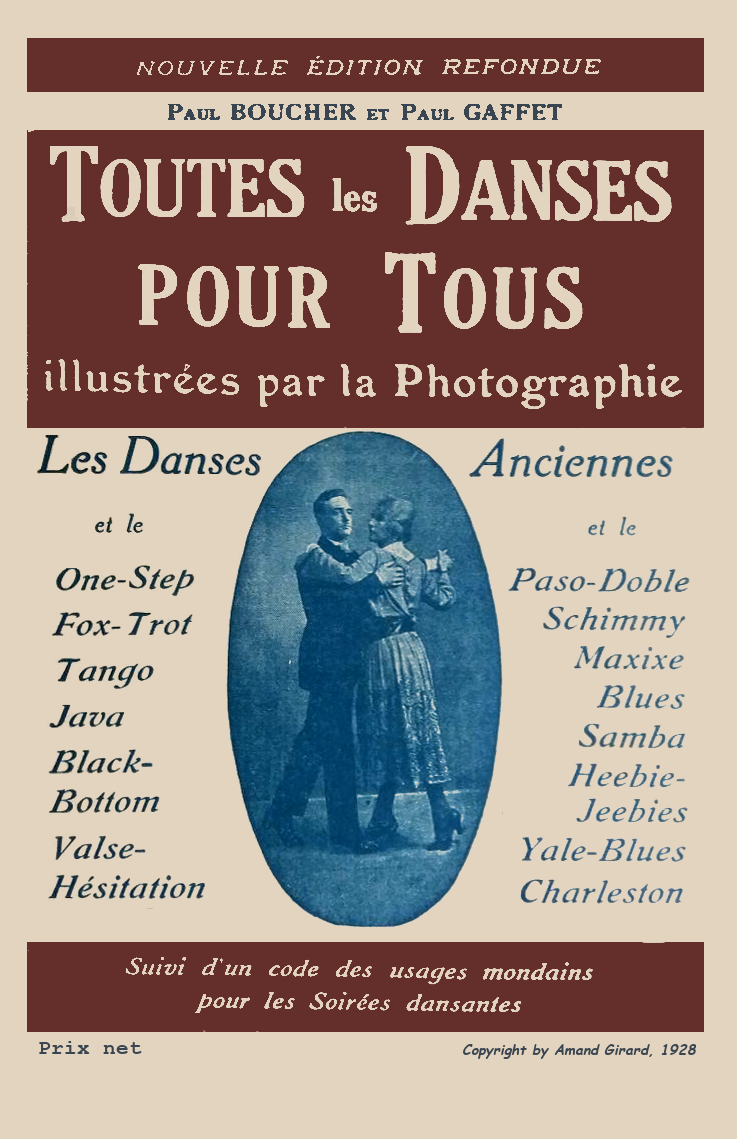
\includegraphics[width=0.5\textwidth]{chapters/cap-historia-sambagafieira/Toutes-les-danses-pour-tous.png}
    \else
    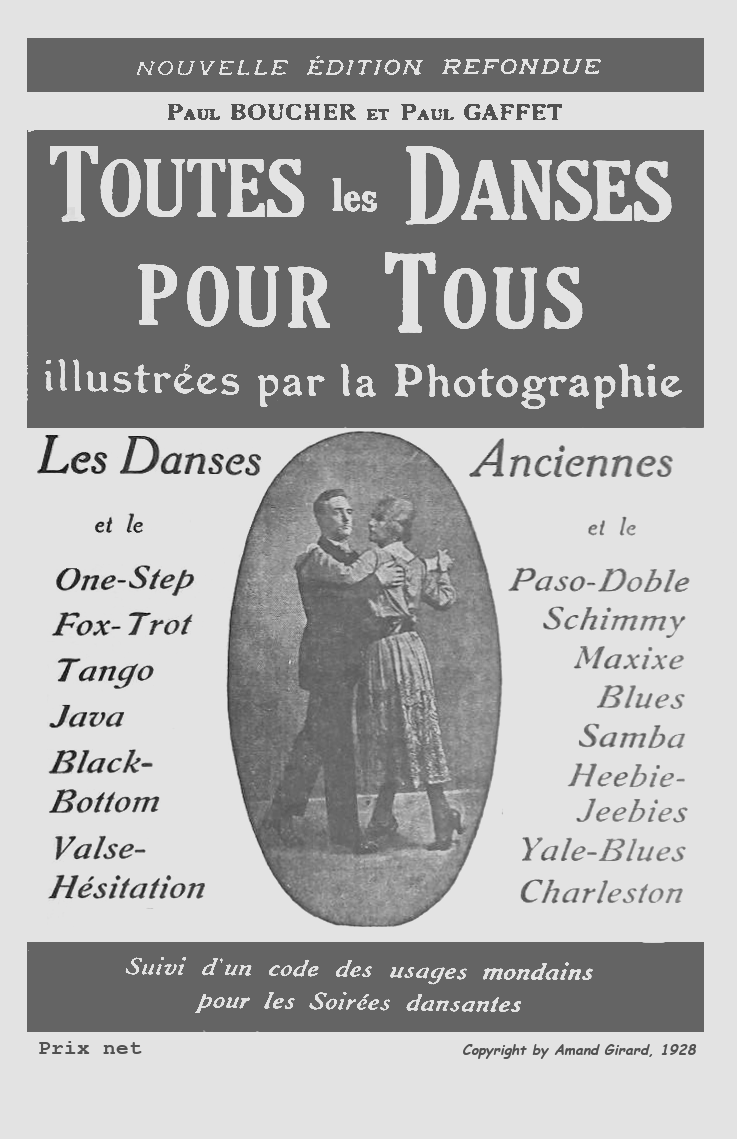
\includegraphics[width=0.5\textwidth]{chapters/cap-historia-sambagafieira/Toutes-les-danses-pour-tous-HSV.png}
    \fi
    \caption{Capa do livro ``Toutes les Danses Pour Tous - Illustrées par la Photographie'' (1928).}
    \label{fig:LivroPaulBoucher}
  \end{figure}


%%%%%%%%%%%%%%%%%%%%%%%%%%%%%%%%%%%%%%%%%%%%%%%%%%%%%%%%%%%%%%%%%%%%%%%%%%%%%%%%
\subsection{O nascimento do samba internacional}


\begin{description}
\item[1922:] O 18 de novembro de 1921 Duque retorna ao Brasil depois de uma viagem a Paris 
para participar numa competência de dança \cite[pp. 465]{marcondes1977enciclopedia} \cite[pp. 3]{duque1921:a}.
Apos algumas coordenações,
o 29 de janeiro de 1922, Duque novamente viaja\footnote{Graças 
ao financiamento do milionário Armando Guinle \cite[pp. 465]{marcondes1977enciclopedia}.} 
 a Paris para divulgar durante seis meses\footnote{Desde 
12 de fevereiro ate agosto \cite{BASTOS2005}. \cite[pp. 5]{batutas1922:c}} 
o samba e outros ritmos brasileiros, 
junto com os ``Oito Batutas''\footnote{O 
grupo estava dirigido por Pixinguinha e incluía Donga \cite{BASTOS2005}.} 
contratados por ele para esse fim
\cite[pp. 13]{duque1922:a} \cite[pp. 465]{marcondes1977enciclopedia}.
Na França o grupo é rebatizado como ``Les Batutas''\footnote{Os 
``Oito Batutas'' foram reduzidos a sete músicos \cite{BASTOS2005}.},
e teve apresentações principalmente no Shéhérazade, 
baixo a direção de Duque \cite[pp. 465]{marcondes1977enciclopedia} \cite{BASTOS2005};
existem varias referencias a estas apresentações, nos jornais franceses, pelo menos desde fevereiro,
ate abril de 1922, elogiando e promovendo as apresentações 
\cite[pp. 5]{batutas1922:a} \cite[pp. 4]{batutas1922:b} \cite{batutas1922:d},
como por exemplo a mostrada na Figura \ref{fig:LesBatutas}.


  \begin{figure}[h!]
    \centering
    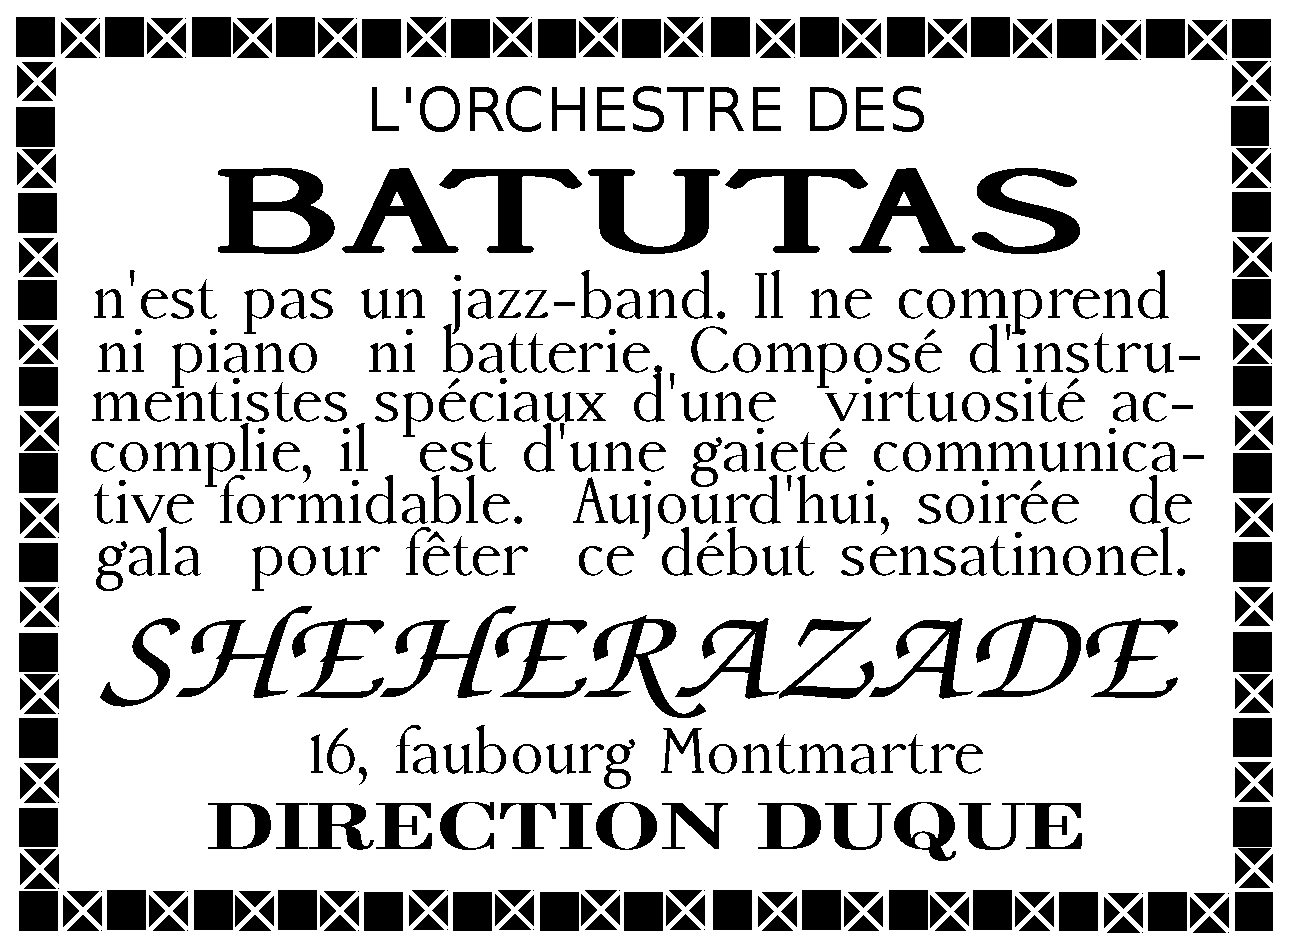
\includegraphics[width=0.5\textwidth]{chapters/cap-historia-sambagafieira/batutas.eps}
    \caption{Anuncio da orquestra dos ``Batutas'' no jornal ``Le Gaulois'' do dia 16 de fevereiro de 1922 \cite[pp. 4]{batutas1922:b}.}
    \label{fig:LesBatutas}
  \end{figure}

\item[1928:] Apos o trabalho feito em 1922 por Duque e os oito batutas, e o constante intercambio cultural entre Brasil e França, 
o samba ficou presente no consciente coletivo do povo parisiense.
No livro ``The Complete Book of Ballroom Dancing'' (1992) se menciona que foi ao redor de 1923
em França, que o ``samba de salão'' (a dança samba internacional) surge \cite[pp. 45]{stephenson1992complete},
como evidencia disto temos que em 1928, 
Paul Boucher e Paul Gaffet publicam  a segunda edição do seu livro de dança:
``Toutes les Danses Pour Tous - Illustrées par la Photographie'',
que inclui o samba além do já conhecidíssimo maxixe, ver Figura \ref{fig:LivroPaulBoucher}.

\item[1925-1929:] Nos Estados Unidos, seguindo o famoso músico brasileiro e líder de orquestra, 
Francisco Marti,
o samba substituiu ao maxixe ao redor de 1925 \cite[pp. 238]{hostetler1942walk}.
Por outro lado, seguindo o livro ``Social Dance: From Dance a While'' (1998),
o samba virou conhecido nos Estados Unidos ao redor de 1929
\cite[pp. 125]{harris1998social}.

\item[1933:] Nos Estados Unidos, o maxixe como expoente de cultura brasileira foi popular 
entre os dançarinos, aproximadamente desde\footnote{Em 
1915 os dançarinos Duque e Gaby fizeram apresentações em New York \cite[pp. 45]{maxixe1915duqueEEUU:1}.} 1910
ate 1920, e foi muito divulgado por Vernon e Irene Castle \cite[pp. 44]{stephenson1992complete}.
Porém, falando de pessoas fora do mundo da dança, 
foi em 1933 que o grande público conheceu o samba e a cultura brasileira no lançamento do filme
``Flying Down to Rio'',
onde Fred Astaire e Dolores del Rio dançam ``Carioca'' \cite[pp. 45]{maxixe1915duqueEEUU:1}.

\item[1938-1939:] Uma exibição de samba foi feita no novembro de 1938
para a ``New York Society of Teachers of Dancing''\footnote{1938, Sociedade de Professores de Dança de Nova York},
e para as pessoas em geral o interesse no samba seria ainda mais estimulado,
na ``Feira Mundial de Nova Iorque''\footnote{1939, World’s Fair in New York} (1939), 
onde o samba foi tocado no pavilhão brasileiro  \cite[pp. 45]{maxixe1915duqueEEUU:1}.

\item[1941:] Carmem Miranda divulgaria também o samba no
 filme de comédia musical ``That night in rio'' (1941) \cite[pp. 45]{maxixe1915duqueEEUU:1}.

\item[1944:] O filme musical ``Brazil'' (1944) é lançado em Hollywood,
onde o ``Soundtracks'' está a cargo do Ary Barroso;
isto apos o exito da música ``Brazil''\footnote{A 
música ``Brazil'' é na verdade ``Aquarela do Brasil'' (1939) 
\cite[pp. 73]{diniz2006almanaque} \cite[pp. 128]{perna2002samba} \cite[pp. 77]{fenerick2005nem}.} 
escrita por ele \cite[pp. 45]{maxixe1915duqueEEUU:1}.

\end{description}

Mais informação sobre o estilo de dança samba internacional na Seção \ref{subsec:DancaSambaInternacional}.
%É criado o estilo de samba internacional \cite[pp. 78]{shaw2018tropical}.

%%%%%%%%%%%%%%%%%%%%%%%%%%%%%%%%%%%%%%%%%%%%%%%%%%%%%%%%%%%%%%%%%%%%%%%%%%%%%%%%
\section{Samba de gafieira (dança)}
\index{Dança!Samba de gafieira}
O samba de gafieira, como dança, descende principalmente do maxixe (dança),
que a sua vez foi gerado  pela união do  lundu, 
a polca e outras danças europeias.
Assim, misturando o maxixe com a ginga, e o ritmo de outras danças africanas, 
é que se obteve o samba dançado nas gafieiras \cite[pp. 139]{perna2002samba}, também chamado
samba de salão ou samba carioca \cite[pp. 50]{fornaciari1947aprender},
atualmente entenderíamos a este samba como o samba de gafieira primigênio\footnote{
Primitivo; primordial; o primeiro da sua espécie. = PRIMÍGENO \cite{priberamprimigenio}.
}.




A Figura \ref{fig:formuladosambagafieira} mostra a árvore genealógico do samba de gafieira,
visto quando o samba (música) fez sua aparição nos salões de dança denominados já no \AnoLivro~ como gafieiras.
\begin{figure}[h]
  \centering
  \begin{subfigure}[b]{0.52\textwidth}
    \centering
    \includegraphics[width=\textwidth]{chapters/cap-historia-sambagafieira/sambagafieiraformula.eps}
    \caption{Formação dos primeiros sambas dançados nas gafieiras ou samba de gafieira (primigênio).}
    \label{fig:formuladosambagafieira}
  \end{subfigure}
  ~~
  \begin{subfigure}[b]{0.37\textwidth}
    \centering
    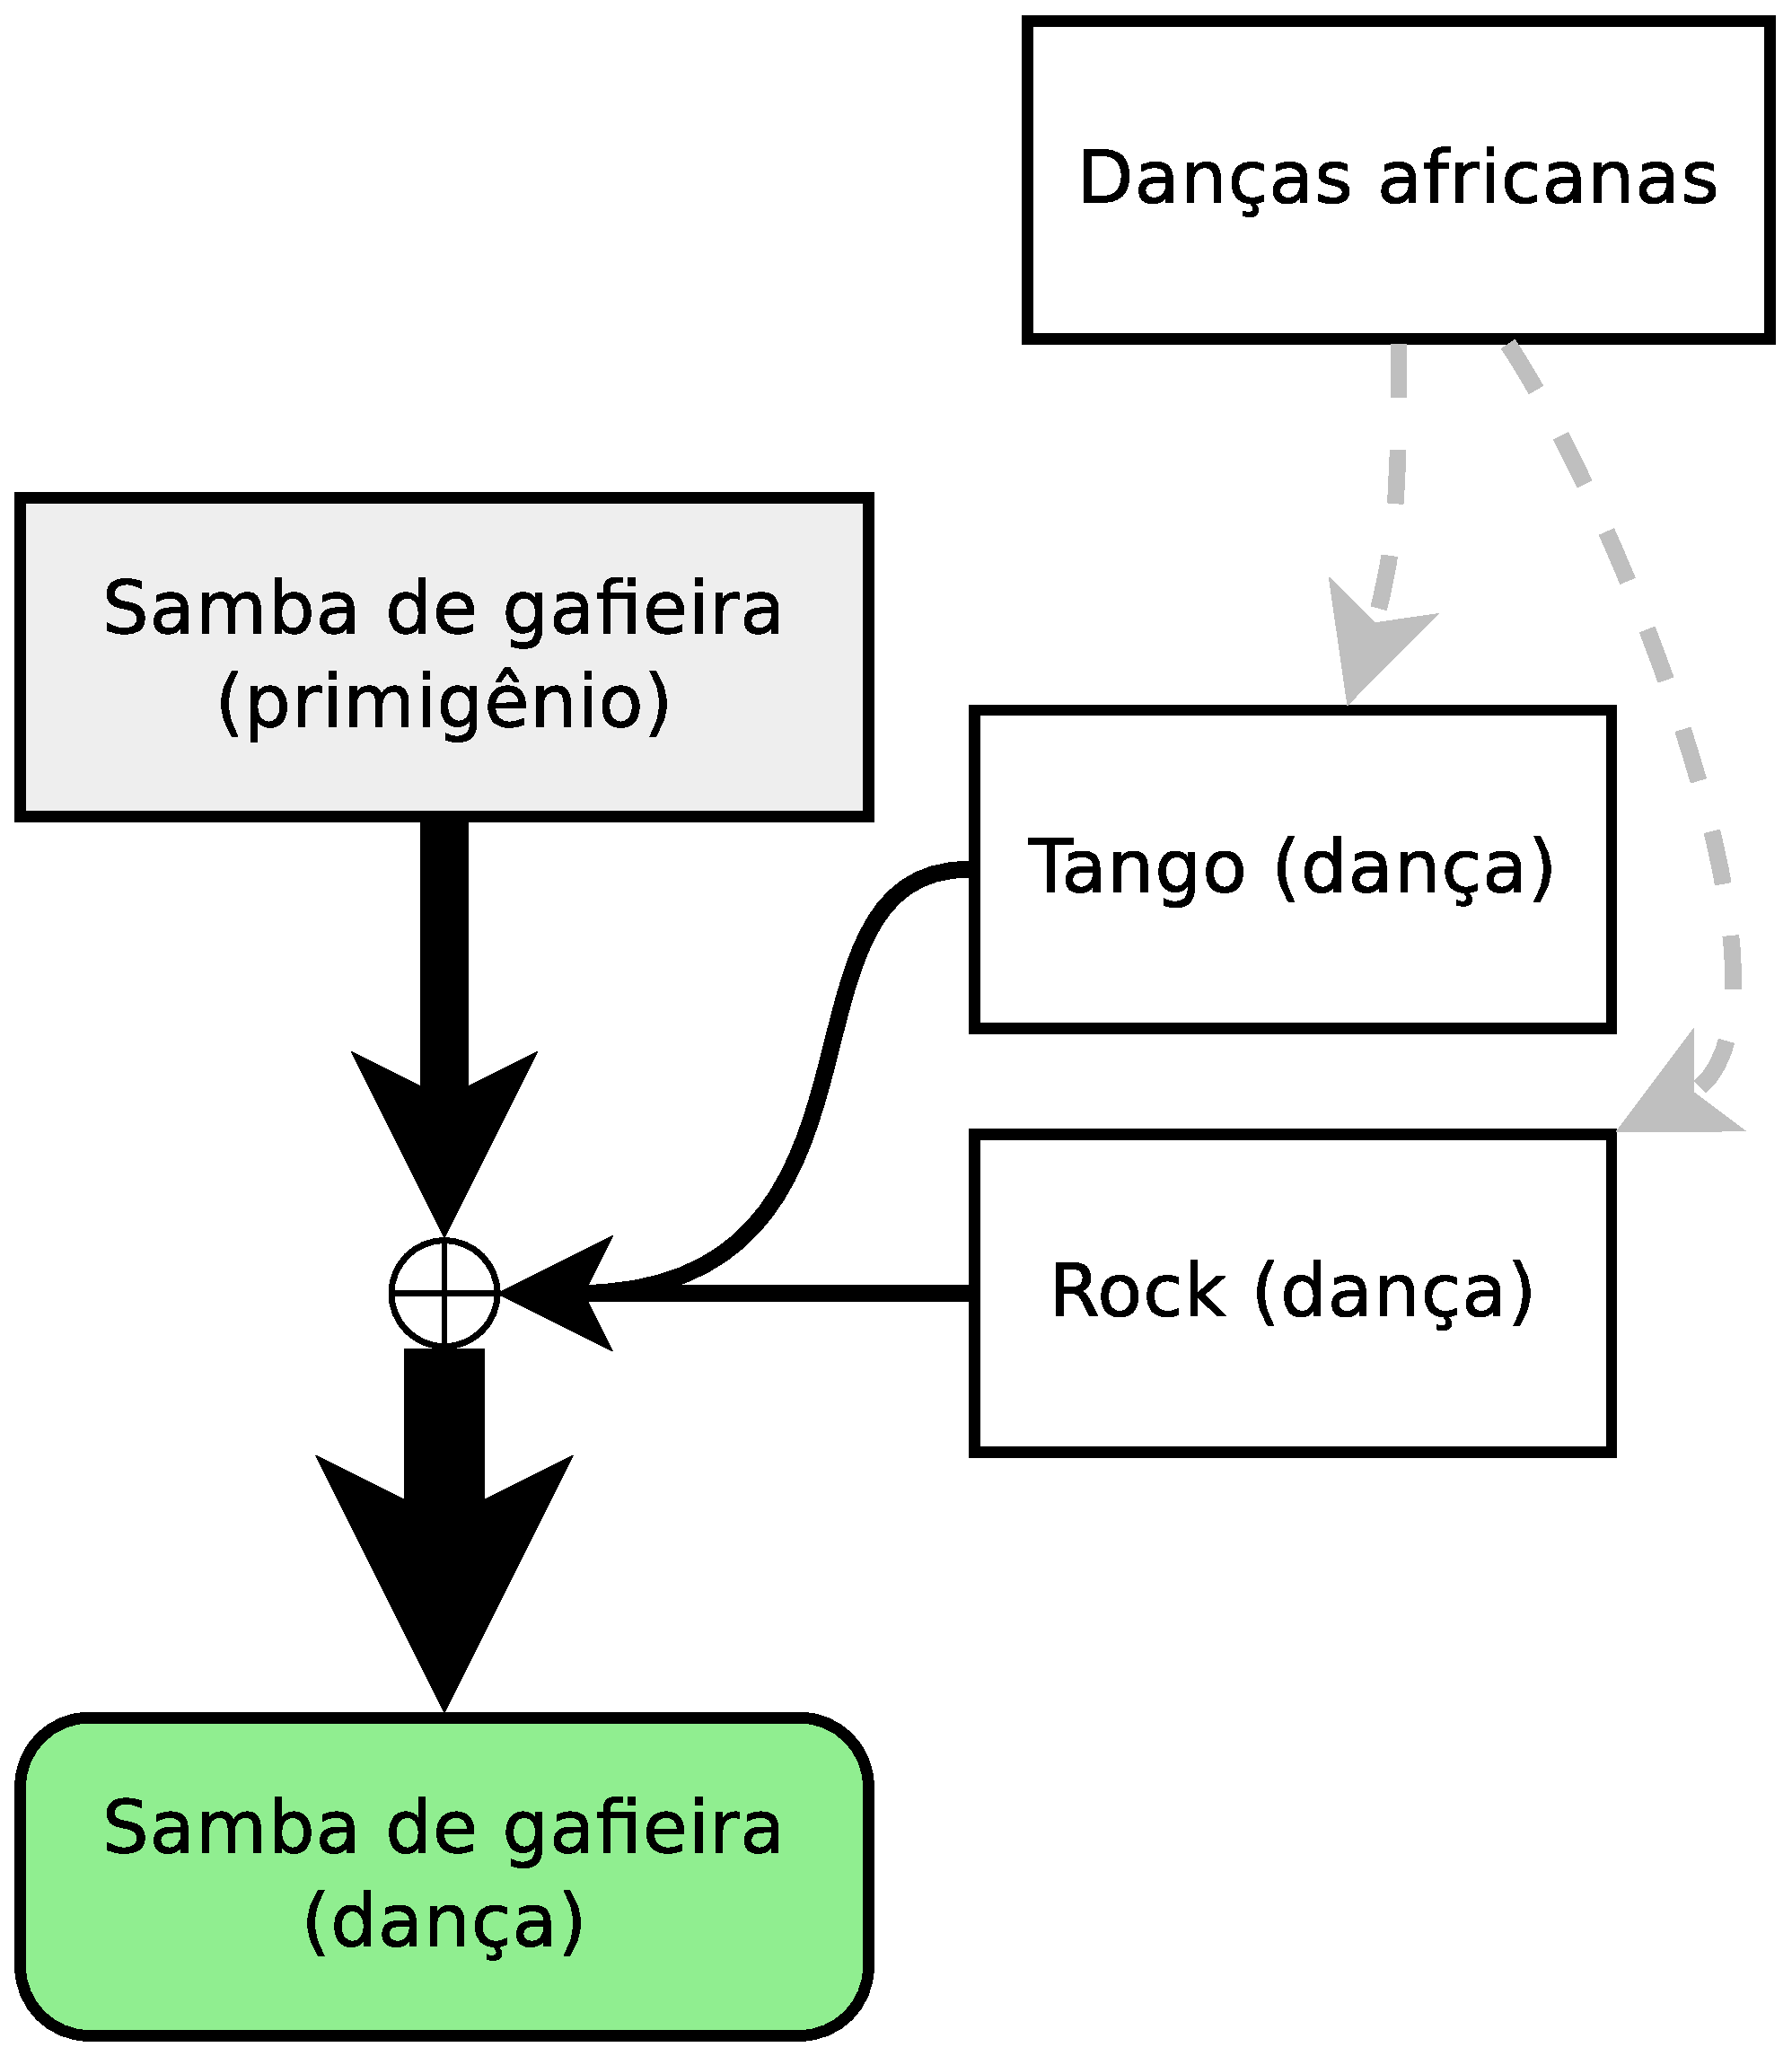
\includegraphics[width=\textwidth]{chapters/cap-historia-sambagafieira/sambagafieiraformula2.eps}
    \caption{Formação do samba de gafieira (atual).}
    \label{fig:formuladosambagafieira2}
  \end{subfigure}
\caption{Formula da criação do samba de gafieira.}
\label{fig:formuladosambagafieiraall}
\end{figure}


No janeiro de 1922, o professor de dança Duque junto com os ``Oito Batutas'', 
viaja a Paris para divulgar o samba e outros ritmos brasileiros
\cite[pp. 13]{duque1922:a} \cite[pp. 465]{marcondes1977enciclopedia},
pode-se deduzir que para esta época já existia algum tipo de forma de dançar o samba nos salões, 
pelo menos algum estilo próprio de Duque,
para ser apresentado na Europa. Isto é assim confirmado porque em 1928,
em Paris, se publicava a segunda edição do livro de dança de Paul Boucher e Paul Gaffet,
titulado
``Toutes les Danses Pour Tous - Illustrées par la Photographie'',
que incluia o samba além do já conhecidíssimo maxixe, ver Figura \ref{fig:LivroPaulBoucher}.


O aparecimento do samba nos salões de dança no Brasil, 
foi um grande impacto para as pessoas que frequentavam estes lugares;
sendo considerado um ritmo novo e ligeiro,
que desagradou aos bailarinos de maior idade e menos ágeis \cite[pp. 6 - cad. B]{entrevistajuliojournalbrasil1}.
O senhor, Júlio Simões, Administrador da ``Kananga do Japão'' e posteriormente socio
do ``Elite Club'', chegou a temer pelo futuro do seus empreendimentos; porém, para sorte dele, 
o samba fez muito sucesso no Elite,
e passou a ser considerado vestibular indispensável para qualquer pessoa que pretendesse ser bailarino, 
compositor ou instrumentista \cite[pp. 6 - cad. B]{entrevistajuliojournalbrasil1}.

Pode-se estabelecer o ingresso do samba aos salões de dança no Brasil numa época anterior e próxima da década de 1930,
dado que Júlio Simões, trabalhou na ``Kananga do Japão'' ate o ano de 1929 \cite[pp. 3 - cad. 3]{juliosimoes}  
\cite[pp. 11]{eliteinaugura} \cite[pp. 1 - cad. B]{gafieira2000reis}, pelo que sua preocupação sobre o samba 
nesse salão de dança deve ser anterior a essa data, porém, não muito atrás dado que 
suas preocupações ainda eram vigentes na sua época no ``Elite Club'' 
que inciou em 1930 \cite[pp. 11]{eliteinaugura} \cite[pp. 3 - cad. 3]{juliosimoes} \cite[pp. 10]{simoesjournalbrasil1}.

\PRLsep{Os sambas nos salões em 1940}

O samba dançado nas gafieiras se firmou na década de 1940 \cite[pp. 142]{perna2002samba}. 
Em palavras do Prof. de dança Gino Fornaciari, 
a dança do samba praticada nos salões ou samba carioca (anterior a 1947 \cite[pp. 50]{fornaciari1947aprender}), 
 tinha um parecido com o Foxtrot e a Rumba, se dançava numa música sincopada com compasso binário,
sendo esta dança a preferida do mulato brasileiro
%sendo este estilo de dança de salão que nasceu na \hyperref[ref:batucadadanca]{\textbf{batucada}} 
%de pretos que descia à cidade na época das festas 
\cite[pp. 50-51]{fornaciari1947aprender}.


Na década de 1940 o samba dançado nos salões 
tinha 3 modalidades, samba-canção, samba-batucada e o samba liso \cite[pp. 58]{freitas1959danca} \cite[pp. 142-143]{perna2002samba} 
\cite[pp. 51]{fornaciari1947aprender}\cite[pp. 51]{fornaciari1950aprender}.

\begin{figure}[h]
    \centering
    \begin{subfigure}[b]{0.7\textwidth}
        \centering
        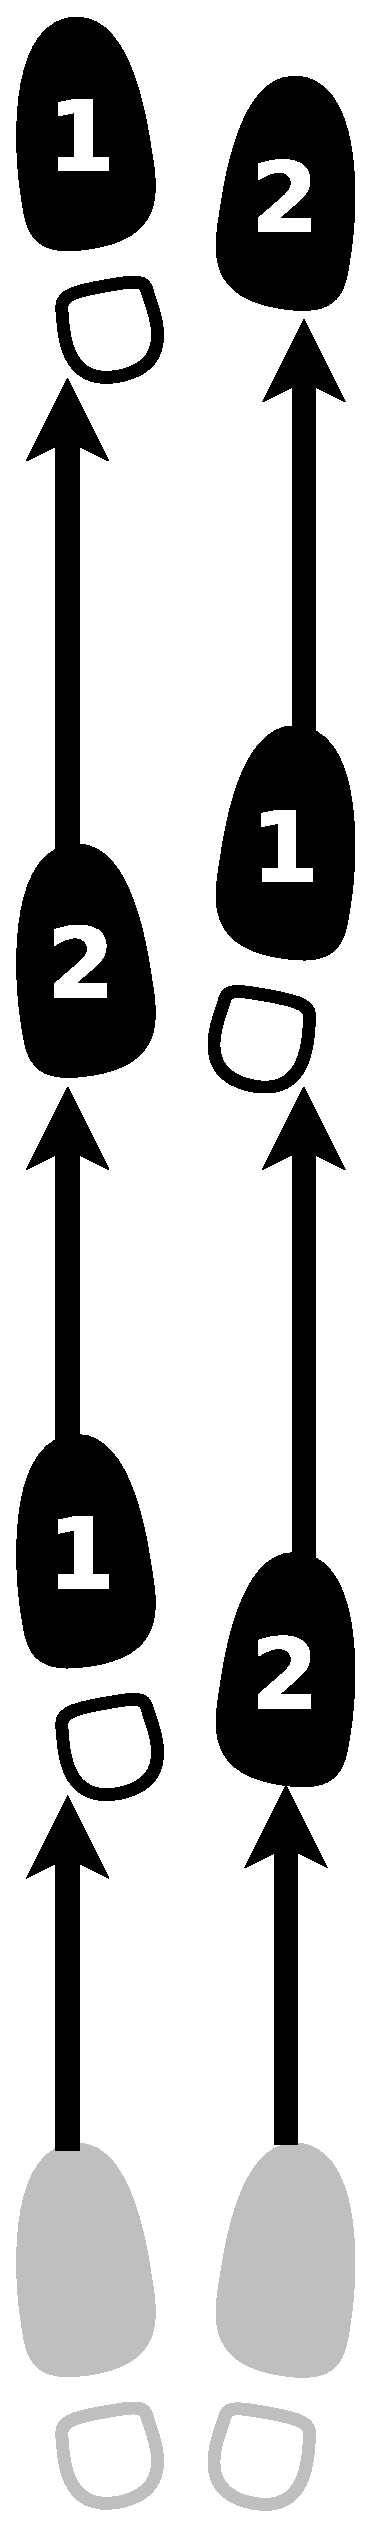
\includegraphics[angle=270,width=0.97\textwidth]{chapters/cap-historia-sambagafieira/samba-cancao-basico-frente.eps}
        \caption{Passo básico para a frente.}
        \label{fig:samba-cancao-basico-frente}
    \end{subfigure}
    ~\\~\\ %add desired spacing between images, e. g. ~, \quad, \qquad, \hfill etc. 
      %(or a blank line to force the subfigure onto a new line)
    
    \begin{subfigure}[b]{0.7\textwidth}
        \centering
	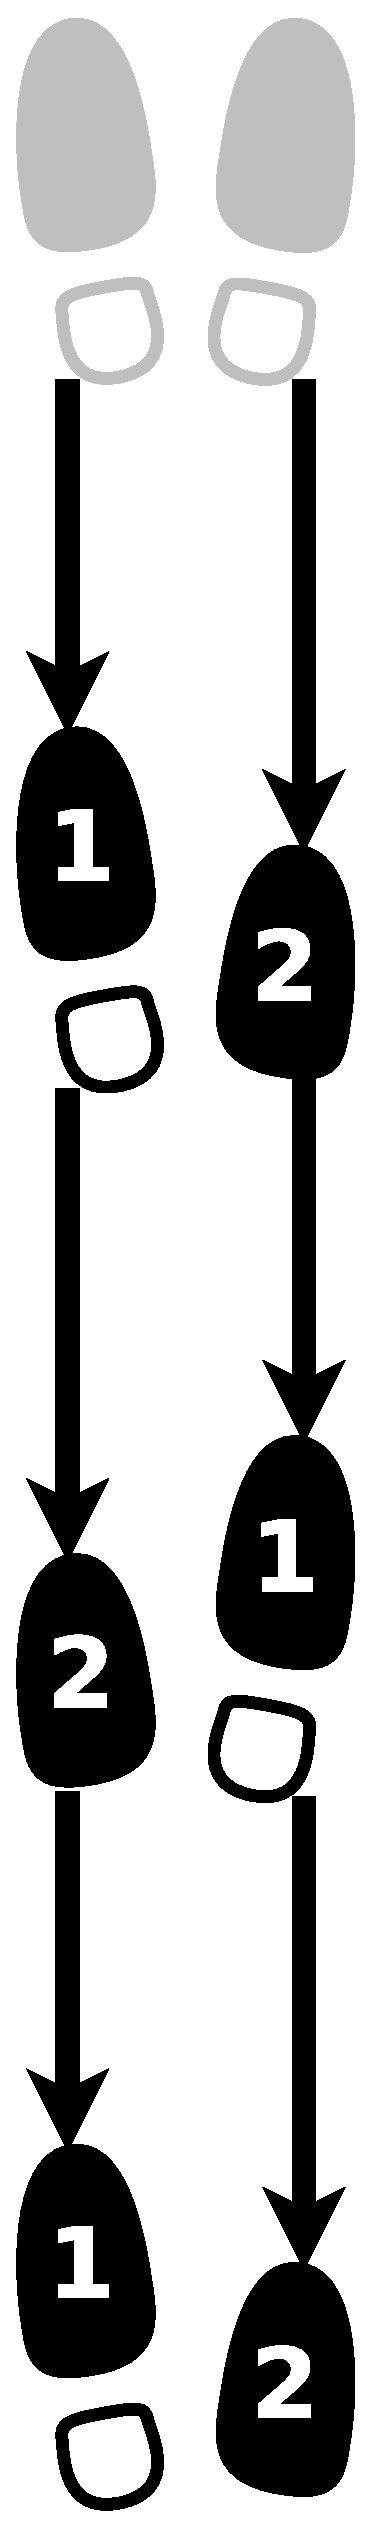
\includegraphics[angle=270,width=0.97\textwidth]{chapters/cap-historia-sambagafieira/samba-cancao-basico-tras.eps}
        \caption{Passo básico para trás.}
        \label{fig:samba-cancao-basico-tras}
    \end{subfigure}
    \caption{Samba-canção da década de 1959.}\label{fig:samba-cancao-basico}
\end{figure}

\begin{itemize}

\item \textbf{Samba-canção (dança):}
\index{Dança!Samba-canção} 
Esta era uma dança com balanços aos lados que se executava de joelhos flexionados,
usando dois movimentos por cada compasso binario \cite[pp. 58]{freitas1959danca} 
\cite[pp. 51]{fornaciari1947aprender} \cite[pp. 143]{perna2002samba}; 
no ano 2001 se considera que este é um modo de dança extinto \cite[pp. 143]{perna2002samba}.
Na Figura \ref{fig:samba-cancao-basico-frente} se mostra o passo básico para a frente do samba-canção,
e na  Figura \ref{fig:samba-cancao-basico-frente} o mesmo movimento para trás,
estes eram usados antes de 1947 e inclusive até o ano de 1959;
em ambos casos os passos constavam de 2 movimentos, e a cor cinza indica a posição inicial \cite[pp. 51]{fornaciari1947aprender} \cite[pp. 59-60]{freitas1959danca}. 



\item \textbf{Samba-batucada:}
\index{Dança!Samba-batucada} 

Existe uma menção sobre este estilo no ``Jornal do Brasil'', no dia 9 de janeiro de 1938,
onde se indica \cite[pp. 4]{musicasambavariasdef1}:
\begin{citando}%%
Tentativas isoladas de puro 
snobismo e ás vezes de compreensão 
inexata da origem da 
musica e dansa, chamam-no de samba jongo, \textbf{samba batucada} ou
pretendem mistura-lo com o fox, -- samba fox ou com a rumba samba-rumba.
\end{citando}



No livro ``Feitiço decente: Transformações do samba no Rio de Janeiro (1917-1933)'' (2001),
se comenta, sobre uma roda do samba, que para o dançarino solista  escolher a seu sucessor podiam
existir duas modalidades, em ``samba liso'' (com umbigada) ou em ``samba duro'' 
(ou batucada) no qual a umbigada é substituída por uma pernada \cite[pp. 109]{sandroni2001feitico}.
Deste comentário pode ser deduzido de onde vem a denominação \textbf{samba-batucada}, 
que surgiu nos salões de dança apos 1930; pois já existia uma tradição na nomenclatura,
em separar duas formas de dançar uma mais leve (a liso) e uma mais brusca (batucada);
assim, a variante de samba no salão que tendia a explorar movimentos muito  gingados, bruscos ou rápidos,
foi nomeado de samba-batucada, em contraposição ao samba liso no qual né se flexionavam os joelhos pra dançar.  



Seguindo o que indicam  os professores de dança Gino Fornaciari e Ivan Freitas,
nos seus respetivos livros, o samba-batucada era desde antes de 1947 e inclusive ate 1959, 
uma dança com balanços que se executava de joelhos flexionados  
e usava 3 movimentos por compasso, que exigia uma maior rapidez, 
especialmente no terceiro movimento que é mais rápido e curto 
\cite[pp. 61]{fornaciari1947aprender} \cite[pp. 58,66]{freitas1959danca};
seguindo essa descrição, 
podemos teorizar que o samba-batucada se dançava seguindo uma distribuição de tempos,
muito parecida ao ritmo do baião de 1949 \cite{CORTES2014}.
Na Figura \ref{time:sambabatucada} se exemplifica a distribuição de tempos do ritmo de baião (1949) em relação ao uso dos pés usando as pissadas que indicam os professores de dança Gino Fornaciari e Ivan Freitas.
\begin{figure}[H]
\centering
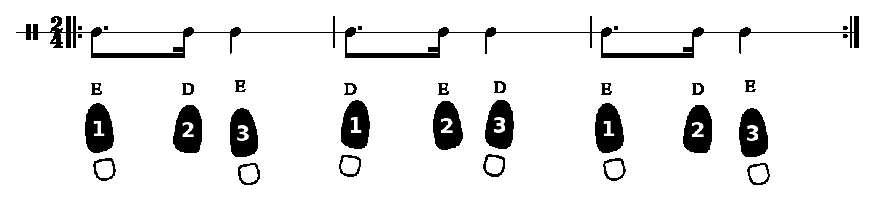
\includegraphics[width=\textwidth]{chapters/cap-historia-sambagafieira/sambabatucada.eps}
\caption{Ritmo das pisadas no samba-batucada.}
\label{time:sambabatucada}
\end{figure}

\parbox[t]{\dimexpr\textwidth-\leftmargin}{%
\begin{wrapfigure}{r}{0.4\textwidth}
  \vspace{-10pt}
  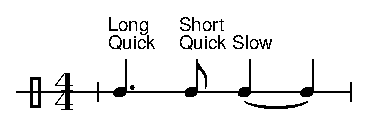
\includegraphics[width=0.38\textwidth]{chapters/cap-historia-sambagafieira/samba-internacional-timming.eps}
  \caption{Samba internacional, pp. 176 do livro ``How to dance'' (1942).}
  \vspace{-10pt}
  \label{timming:samba-internacional:a}
\end{wrapfigure}
A descrição do movimento, a qual indica que a terceira pisada é mais rápida,
é um pouco ambígua, 
pois não fica evidente si refere-se à velocidade com a que o pé se desloca ate tocar o chão e contar 3,
ou refere-se à velocidade do movimento para dar o seguinte passo, apos ter pisado 3;
porém, 
independentemente da assinação de números escolhida, 
a Figura \ref{time:sambabatucada} cumpre com as proporções na distribuição de tempos 
indicada pelos professores Fornaciari e Freitas para o samba-batucada.
}
Assim, a teoria planteada aqui, sobre a distribuição de tempos para o samba batucada, 
é concordante com o achado em livros sobre o $\ll$samba internacional$\gg$  
dessa época e posteriores\footnote{Nas referencias bibliográficas tenho achado publicações desde 1945 ate 1998,
indicando uma distribuição de tempos para o samba internacional como a apresentada na Figura \ref{time:sambabatucada}
\cite[pp. 7,176]{wright1945dance} \cite[pp. 193]{white1953dancing} \cite[pp. 69]{stephenson1992complete} \cite[pp. 125]{harris1998social}.}
\cite[pp. 7,176]{wright1945dance} \cite[pp. 193]{white1953dancing} \cite[pp. 69]{stephenson1992complete} \cite[pp. 125]{harris1998social},
os quais indicam uma distribuição de tempos para o samba internacional como as mostradas nas Figura \ref{time:sambabatucada} e \ref{timming:samba-internacional:a};
pelo que podemos intuir que o samba-batucada ainda tinha essa caraterística em comum com seu ``primo'' internacional.

\begin{comment}
X: 1 % start of header
K: C stafflines=1 % scale: C major
M: 4/4 %meter - compasso
V:1 clef=perc stem=up %name="Pauta com clave de fá"   sname="Pauta com clave de fá"
[V:1] |"Long\nQuick"B3 "Short\nQuick"B1 "Slow"(B2 B2)|
\end{comment}


Sobre os passos de samba-batucada usados desde antes de 1947: 
A Figura \ref{fig:samba-batucada-basico-frente}  mostra o passo básico para a 
frente, do samba-batucada, 
e na  Figura \ref{fig:samba-batucada-basico-tras} temos o mesmo movimento para trás;
em ambos casos se usam passos em grupos de 3; a cor cinza indica a posição inicial \cite[pp. 61-62]{fornaciari1947aprender} \cite[pp. 63]{freitas1959danca}. 
\begin{figure}[h]
    \centering
    \begin{subfigure}[b]{0.7\textwidth}
        \centering
        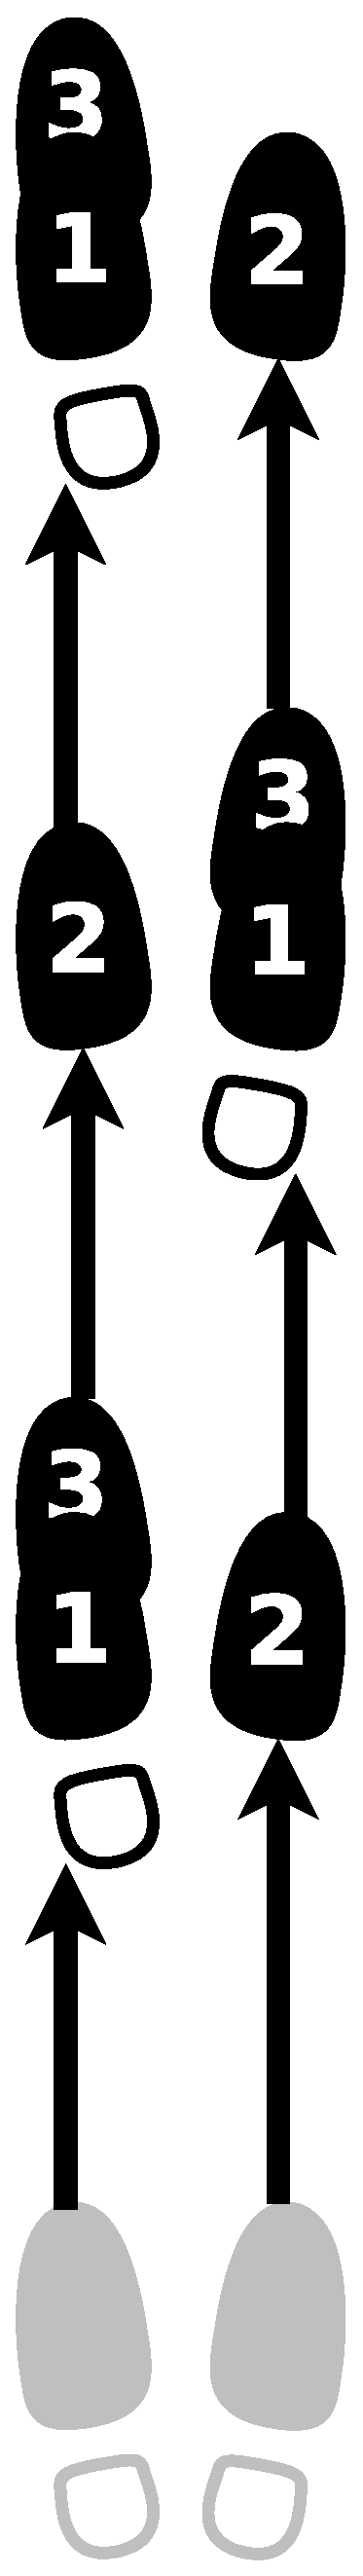
\includegraphics[angle=270,width=0.97\textwidth]{chapters/cap-historia-sambagafieira/samba-batucada-basico-frente.eps}
        \caption{Passo básico para a frente.}
        \label{fig:samba-batucada-basico-frente}
    \end{subfigure}
    ~\\~\\ %add desired spacing between images, e. g. ~, \quad, \qquad, \hfill etc. 
      %(or a blank line to force the subfigure onto a new line)
    \begin{subfigure}[b]{0.7\textwidth}
        \centering
	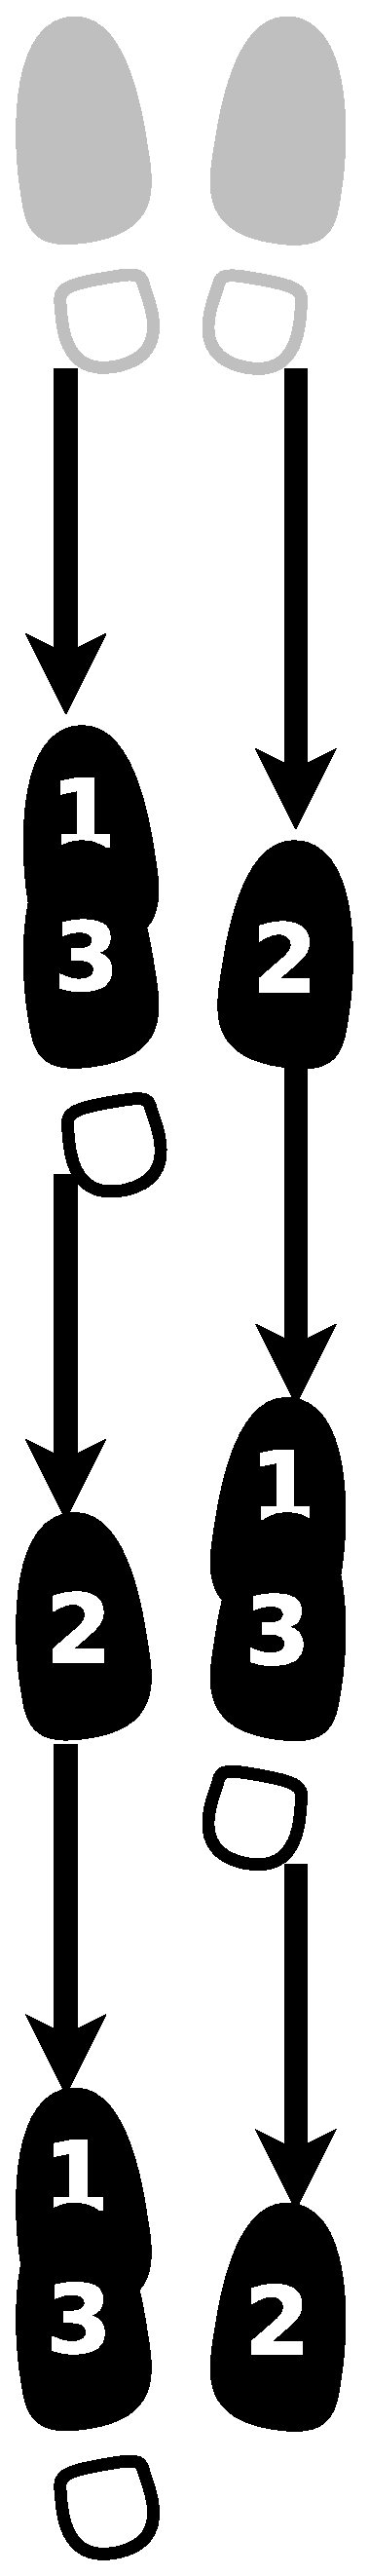
\includegraphics[angle=270,width=0.97\textwidth]{chapters/cap-historia-sambagafieira/samba-batucada-basico-tras.eps}
        \caption{Passo básico para trás.}
        \label{fig:samba-batucada-basico-tras}
    \end{subfigure}
    \caption{Samba-batucada da década de 1959.}\label{fig:samba-batucada-basico}
\end{figure}

Outros passos conhecidos no ano de 1947, para este estilo de samba, tem nomes como: 
o pião, o balão, a cortada, a meia cortada, a joelhada, a patineta, e outros \cite[pp. 66]{fornaciari1947aprender}.
Para o Prof. Fornaciari, em São Paulo no ano de 1947 o pião e o balão são o mesmo movimento, 
sendo este o movimento mais importante do samba-batucada;
e a diferença do pião de \AnoLivro, que se executa tradicionalmente em sentido horário,
o pião de 1947 se executava em sentido anti-horário \cite[pp. 68,72]{fornaciari1947aprender} 
\cite[pp. 73]{fornaciari1950aprender}.

Seguindo o Prof. Fornaciari, além dos estilos dançados nos salões, 
no ano de 1950, também existiam as danças estilizadas que estavam orientadas 
para serem executadas em teatros \cite[pp. 149]{fornaciari1950aprender}. 
No caso do samba estilizado, este precisava de maior esforço físico dos dançarinos 
além de ser uma dança com maior flexibilidade, jogo de pernas, e com passos mais variados.
Por exemplo, no livro ``Como aprender a dançar'' (1950), temos um movimento que inicia com o condutor no abraço de dança,
e depois este dá uma patinada ou passo para atrás com a perna esquerda 
ao mesmo tempo que eleva ao seguidor \cite[pp. 160-1961]{fornaciari1950aprender};
este movimento  é muito similar a outro atual, chamado ``Elevador'', 
que é muito conhecido no samba de gafieira de \AnoLivro.
Nessa mesma página se explica outro movimento, esta vez chamado de ``cortada'', 
que não é outra coisa que uma pernada (presumivelmente só um contato leve) que o condutor da com sua perna esquerda,
sobre a perna direita do seguidor, um pouco abaixo do quadril\footnote{
Pessoalmente lembro ter visto este movimento ao contrario, quando um seguidor da esta pernada 
sobre a perna do condutor, um pouco abaixo do quadril, e o condutor aproveita para fazer uma sacada de perna,
inclusive tenho lembranças de telo visto no tango.}.
O livro também explica um movimento de samba estilizado chamado ``Joelhada'' \cite[pp. 160-1961]{fornaciari1950aprender}, 
que mas bem é uma posição, sendo esta muito similar à posição de ``Facão'' no samba de gafieira de \AnoLivro,
porém, a posição do abraço é muito mais aberta, de modo que ao não estar colados,
o único ponto de contato entre os pares é a parte interna do joelho. 
Como uma semelhança mais com o facão,
no livro se indica que a joelhada pode ser executada apos o pião (do ano de 1947 que era em sentido anti-horário).
Outro movimento no samba estilizado é a ``calçada'', pela descrição feita no livro,
este movimento, é o que no samba de gafieira de \AnoLivro~ chamaríamos ou associaríamos com o ``Balão'' \cite[pp. 162]{fornaciari1950aprender},
com a diferença de que na versão explicada no livro, este movimento não termina numa ``cadeirinha'',
e simplesmente apos chegar ao lado da perna esquerda do condutor (que era quando acontecia a cadeirinha), 
o seguidor retorna ao lado direito do condutor. 
Finalmente o livro revela,
que o passo básico do samba estilizado é o passo básico do samba-batucada \cite[pp. 163]{fornaciari1950aprender},
assim, o termo samba estilizado indica uma versão melhorada do samba-batucada,
orientado para teatros e apresentações. 

Pela semelhança do samba-batucada com os passos de samba de gafieira de \AnoLivro,
nos passos ``Elevador'', ``Balão'' e ``Facão'', podemos teorizar, de que a modalidade samba-batucada foi
a que finalmente se converteu ou aportou mais ao samba de gafieira atual.
Uma evidencia que sustenta esta ideia, a podemos encontrar no filme ``Aviso aos navegantes'' (1950) \cite[min. 40:35]{AtlantidaDance},
no qual a partir do minuto \href{http://www.bcc.org.br/filmes/443382}{40:35} podemos ver uma apresentação de samba de salão (sem especificar a modalidade),
na qual os dançarinos fazem movimentos que no \AnoLivro~chamaríamos de elevador e balão; 
além de varias sequencias de movimentos estilizados semelhantes aos descritos no livro ``Como aprender a dançar'' (1950) do Prof. Fornaciari \cite[pp. 163]{fornaciari1950aprender}.
Por outro lado pode-se perceber movimentos de pés, 
com uma distribuição de tempos com uma semelhança como a descrita na Figura \ref{time:sambabatucada},
dando maior força à hipótese de que essa era a distribuição de tempos para o samba-batucada nessa época. 
%O samba-batucada é o samba de gafieira (primigênio) \cite[pp. 143]{perna2002samba}.

\item \textbf{Samba liso:}
\index{Dança!Samba liso}

Era uma dança com balanços que se dançava sem flexionar os joelhos;
este é um estilo de dança que perdura ainda ate nossos 
dias \cite[pp. 58,62]{freitas1959danca} \cite[pp. 61]{fornaciari1950aprender} \cite[pp. 143]{perna2002samba}, 
para mais detalhes ver a Seção \ref{subsec:sambalisodef}.
\end{itemize}

\subsection{Evolução do samba nos salões}

Com o passar dos anos foram agregados elementos de outras danças a esse primitivo, samba de gafieira;
por exemplo, movimentos do tango e do rock \cite[pp. 142]{perna2002samba}, 
obtendo assim a forma de dança que vemos hoje em dia, ver Figura \ref{fig:formuladosambagafieira2}.

Asim, podemos falar do samba de gafieira como dança, só apos da aparição do samba nos
salões de dança abertos ao público, e a partir da criação do termo gafieira pra definir a estes lugares.
Com a mistura destes dois acontecimentos obtemos o termo, samba de gafieira,
que iniciou seu caminho na dança, mas como uma descrição do âmbito da dança (e da música), que como nome próprio.
Porém, a formação dos movimentos e corporalidade desta dança tem um caminho que data desde muito tempo atrás,
desde os batuques, dos morros e das rodas.


A primeira referencia achada\footnote{Que não quer dizer a primeira existente.} 
na ``Hemeroteca Digital Brasileira'' da Fundação Biblioteca Nacional,
foi na ``Revista da Semana''(RJ), no dia 25 de dezembro de 1948,
onde na seção ``Eros Volusia'', subseção ``O pitoresco da excursão'', se indica \cite[pp. 48]{sambagafieirarefbn}
\begin{citando}
Ensinando o samba aos ministros da República, 
fazendo o povo vibrar com o \textbf{samba de gafieira}, entusiasmando
o meio intelectual com seu francês muito doce,
contando coisas desconhecidas aos dançarinos francêses,
fazendo a dança brasileira figurar nos Archives Internationales de la Danse.
Eros Volusia satisfez o grande ideal de sua vida artística, sentindo-se contente
com o que realizou na França, embora a Europa não dê dinheiro a ninguém.
O lucro artístico é que compensa.
\end{citando}


A Figura \ref{fig:sambagafieiracrono} mostra a cronologia do uso do termo samba de gafieira. 

\begin{figure}[h]
  \centering
    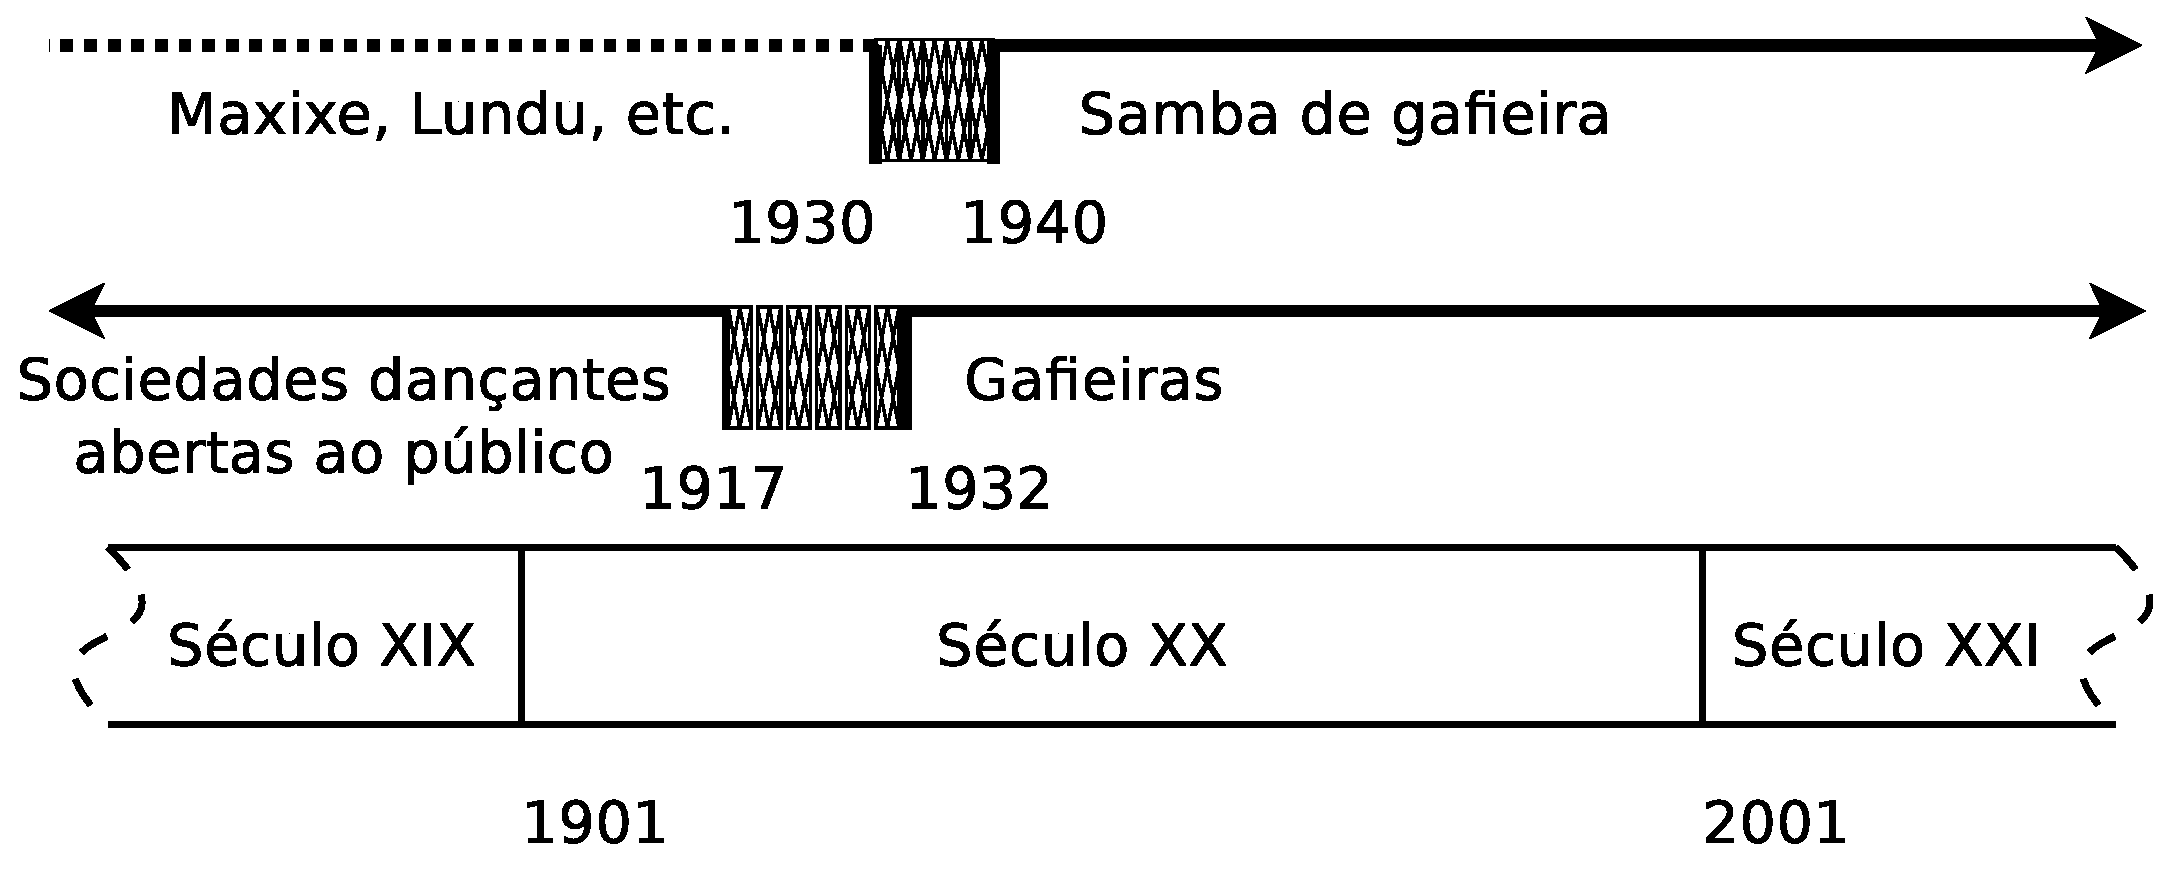
\includegraphics[width=1.0\textwidth]{chapters/cap-historia-sambagafieira/gafieira-crono.eps}
  \caption{ Cronologia da formação do samba de gafieira.}
\label{fig:sambagafieiracrono}
\end{figure}

%%%%%%%%%%%%%%%%%%%%%%%%%%%%%%%%%%%%%%%%%%%%%%%%%%%%%%%%%%%%%%%%%%%%%%%%%%%%%%%
%\clearpage
\section{Música para dançar samba de gafieira}
\label{subsec:gafieiradancaestilos}

Entre os estilos musicais em que o samba de gafieira (dança) se adapta bem, 
estão alguns dos subgêneros do samba; assim,
aqui mencionaremos algumas músicas que por sua graça, estilo e alegria,
a meu entender, podem ser dançados usando o samba de gafieira. Porém, 
estas músicas não pretendem ser máximos expoentes representativos do subgênero em que estão agrupados;
e sim uma indicação ou orientação ao leitor, 
para treinar sua dança usando músicas em que possa ser mais confortável a experiencia.

\begin{itemize}
\item \textbf{Samba de gafieira (música)}
\begin{example} ~
\begin{itemize}
%\item ``Samba de padua'' interpretado pelo grupo Turma da Gafieira.
\item ``Samba de morro'' interpretado pelo grupo Turma da Gafieira.
%\item ``Piston da gafieira'' de Billy Blanco, interpretado por Jorge Beiga.
\item ``Piston da gafieira'' de Billy Blanco, interpretado por Zeca pagodinho \cite{barbosa2014zeca}.
\item ``Beija-me'' de Roberto Martins e Mário Rossi, interpretado por Zeca pagodinho \cite{barbosa2014zeca}.
\item ``Pisei num despacho'' de Geraldo Pereira e Elpídio Viana, interpretado por Zeca pagodinho \cite{barbosa2014zeca}.
%\item ``Tive sim'' de Cartola, interpretado por Zeca pagodinho \cite{barbosa2014zeca}.
%\item ``Tarzan, o filho do alfaiate'' de Noel Rosa e Vadico, interpretado por Zeca pagodinho \cite{barbosa2014zeca}.
%\item ``Se você visse'' de Dino 7 cordas e Del Loro, interpretado por Zeca pagodinho \cite{barbosa2014zeca}.
\end{itemize}
\end{example} 

\item \textbf{Samba de breque}
\begin{example} ~
\begin{itemize}
\item ``Baile no elite'' interpretado por Casuarina.
\item ``Eu sou a marrom'' interpretado por Alicione.
%\item ``Hoje sou diferente'' interpretado por Lenita Rodrigues.
\item ``Pra levantar poeira'' interpretado por Bodhar.
\end{itemize}
\end{example} 

\item \textbf{Samba exaltação}
\begin{example} ~
\begin{itemize}
\item ``Aquarela do Brasil'' interpretado por Gal Costa.
\item ``Canta Brasil'' interpretado por Gal Costa.
\item ``Saudosa maloca'' interpretado pelo grupo Demônios da Garoa.
\end{itemize}
\end{example} 


\item \textbf{Pagode paulista (Sambalanço)}
\begin{example} ~
\begin{itemize}
\item ``Cheia de manias''  interpretado pelo grupo Raça Negra.
\end{itemize}
\end{example} 

\item \textbf{Partido alto}
\begin{example} ~
\begin{itemize}
%\item ``A língua'' interpretado por Beto lima.
\item ``Partido alto'' interpretado por Aleh.
\end{itemize}
\end{example} 

\item \textbf{Pagode}
\begin{example} ~
\begin{itemize}
\item ``Trilha do amor''  interpretado pelo Grupo Revelação. 
\item ``A batucada te pegou'' interpretado pelo Grupo Sou Muleke.
\item ``Dança da solidão'' interpretado por Pagode de Mesa do álbum Terra Brasil. 
\item ``Eu e você sempre'' interpretado por Jorge Aragão
\end{itemize}
\end{example} 

\item \textbf{Samba-canção (música)}
\begin{example} ~
\begin{itemize}
\item ``Só louco'' interpretado por Luiz Melodia.
\item ``Você é a fonte'' interpretado por  Quinteto em Branco e Preto.
\item ``Eu quero é sossego'' interpretado por Paulo Moura.
\end{itemize}
\end{example} 

\item \textbf{Bossa nova}
\begin{example} ~
\begin{itemize}
\item ``I don't know (Bossa mix)'' interpretado por Erika do álbum ``I don't know''
\item ``Human nature'' interpretado por Marcela Mangabeira.
\end{itemize}
\end{example} 


\item \textbf{Choro}
\begin{example} ~
\begin{itemize}
\item ``Choro de gafieira'' de Pixinguinha.
\item ``Chorinho de gafieira'' de Astor Silva.
\item ``Noites cariocas'' de Jacob do Bandolim.
\end{itemize}
\end{example} 


\item \textbf{Samba-choro}
\begin{example} ~
\begin{itemize}
\item ``Escurinho'' interpretado por Corina Magalhães.
\item ``Tico tico no fubá'' interpretado por Leci Brandão.
\end{itemize}
\end{example}

\end{itemize}

A Figura \ref{fig:gafieiradancaestilos} mostra um resumo de alguns dos 
subgêneros do samba nos quais pode ser dançado o samba de gafieira.
\begin{figure}[h]
  \centering
    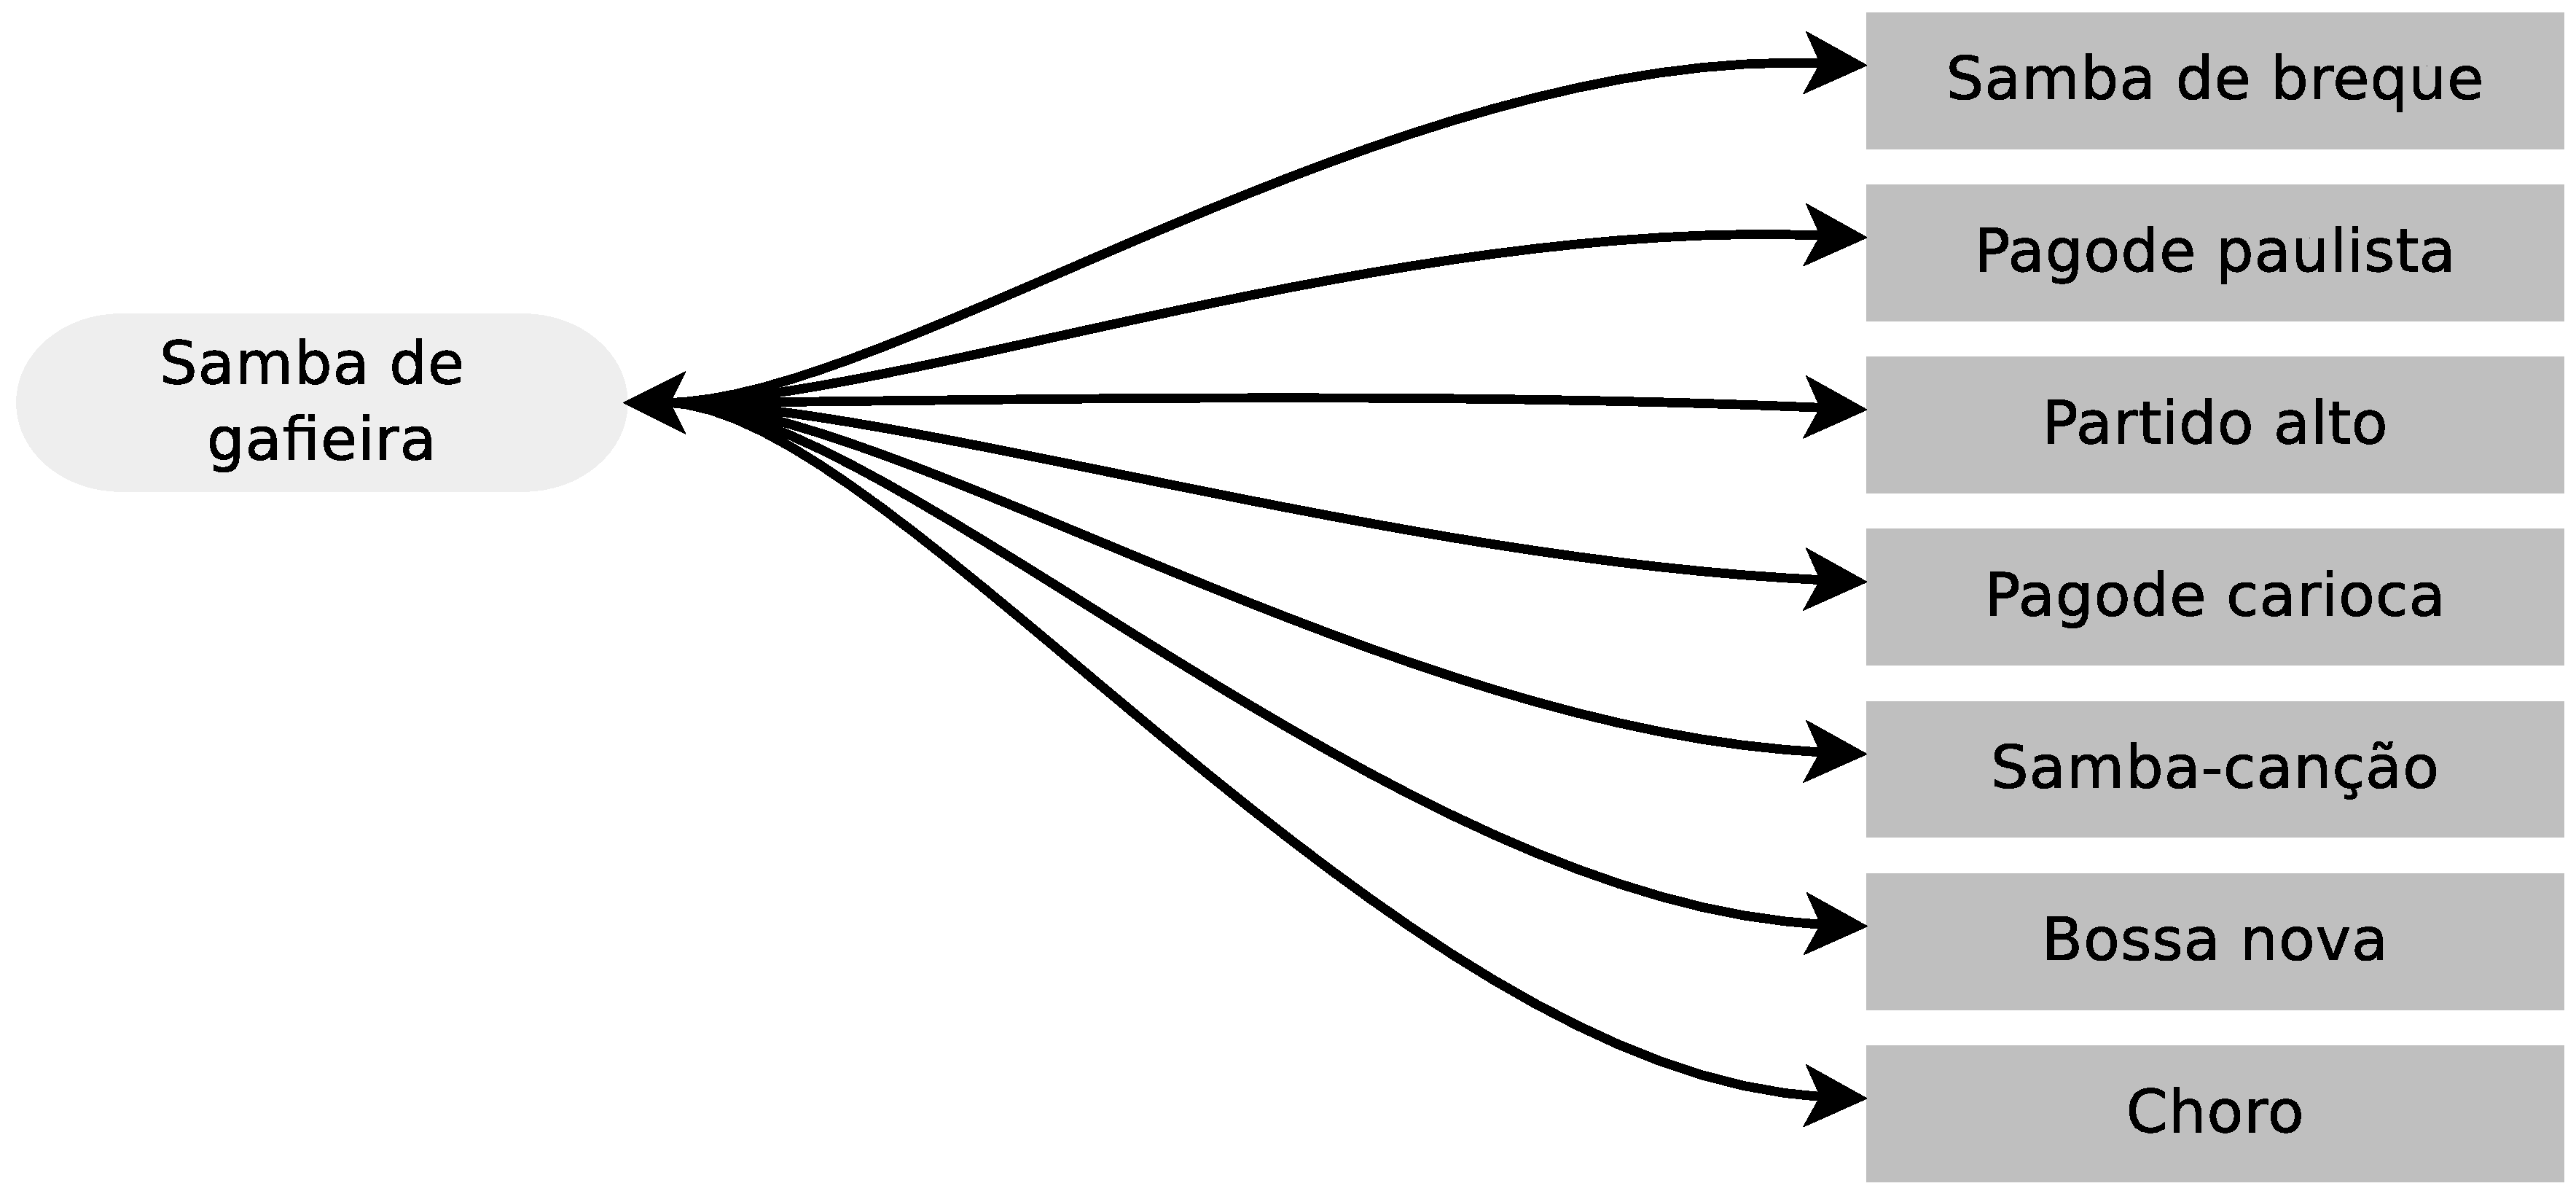
\includegraphics[width=0.9\textwidth]{chapters/cap-historia-sambagafieira/gafieiravcmusica.eps}
  \caption{ Subgêneros do samba nos quais pode-se dançar samba de gafieira.}
\label{fig:gafieiradancaestilos}
\end{figure}

